\documentclass[12pt]{article}
\usepackage{hyperref}
\usepackage[warn]{mathtext}
\usepackage[T2A]{fontenc}
\usepackage[utf8]{inputenc}
\usepackage[russian]{babel}
\usepackage{cite}
\usepackage{amsfonts}
\usepackage{lineno}
\usepackage{subfig}
\usepackage{graphicx}
\usepackage{xcolor}
\usepackage{bm}
\usepackage{graphicx}
\usepackage{amssymb}
\usepackage{hyperref}
\usepackage[left=2cm,right=2cm,top=2cm,bottom=2cm]{geometry}

\DeclareGraphicsExtensions{.png,.jpg}
\date{5 сентября 2021 г.}
\author{Карцев Вадим}
\title{Лабораторная работа 5.1

Измерение коэффициента ослабления потока $\gamma$-лучей в веществе и
определение их энергии}

\begin{document}

\maketitle

\textbf{Цель работы:} измерение коэффициента ослабления потока $\gamma$-лучей
в веществе и определение их энергии.

\vspace{0.3cm}

\textbf{В работе используются:} источник $\gamma$-лучей, свинцовый контейнер с
коллиматорным каналом, набор поглотителей, сцинтиллятор, усилитель
формирователь.

\vspace{1.5cm}

\section{Теоретическая справка}

  Гамма-лучи возникают при переходе возбужденных ядер из одного энергетического
  состояния в длругое, более низкое. Проходя через вещество, пучок $\gamma$-
  квантов постепенно ослабляется. Ослабление происходит по экспоненциальному
  закону:
  $$I = I_0e^{-\mu l}$$ где $$\mu = \frac{1}{l}\log{\frac{N_0}{N}}$$
  Зная количество частиц, прошедших через поглотитель, можем найти коэффициент
  поглощения для данного поглотителя.

\newpage

\section{Определение коэффициента ослабления для разных \\материалов}

  Для нахождения коэффициента поглощения для свинца, алюминия и железа
  воспользуемся установкой
  \begin {figure}[h!]
    \begin{minipage}[h]{0.99\linewidth}
        \center{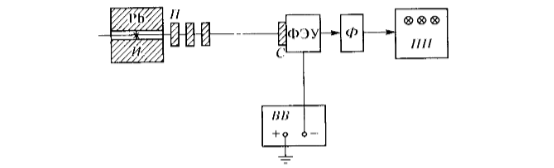
\includegraphics[width = 13cm]{ustanovka.png}}\\
        Рис 1. Схема установки

        \textit{И - источник $\gamma$-лучей, $Pb$ - свинцовый контейнер с
        коллиматорным каналом, $H$ - набор поглотителей, $C$ - сцинтиллятор -
        кристалл $NaI$, Ф - усилитель-формирователь}
    \end{minipage}
    \label {fig:image1}
  \end {figure}

  \vspace{0.2cm}

  Количество зарегестрированных частиц без поглотителя $N = 916099$ шт. за
  $101,9$ секунд.
  Таким образом $N_{0ф} = 899017$ шт.

  Измерили фон, закрыв коллиматорное отверстие цинковой пробкой.
  Количество зарегистрированых частиц фона $N_ф = 2271$ шт.

  Таким образом, без поглотителя за 100 секунд мы регистрируем $N_0 = 896746$
  частиц за вычетом фона.

  \begin {figure}[h!]
    \begin{minipage}[h]{0.49\linewidth}
      Табл 1. Количество частиц, прошедших через свинец за 100 сек.
      \center{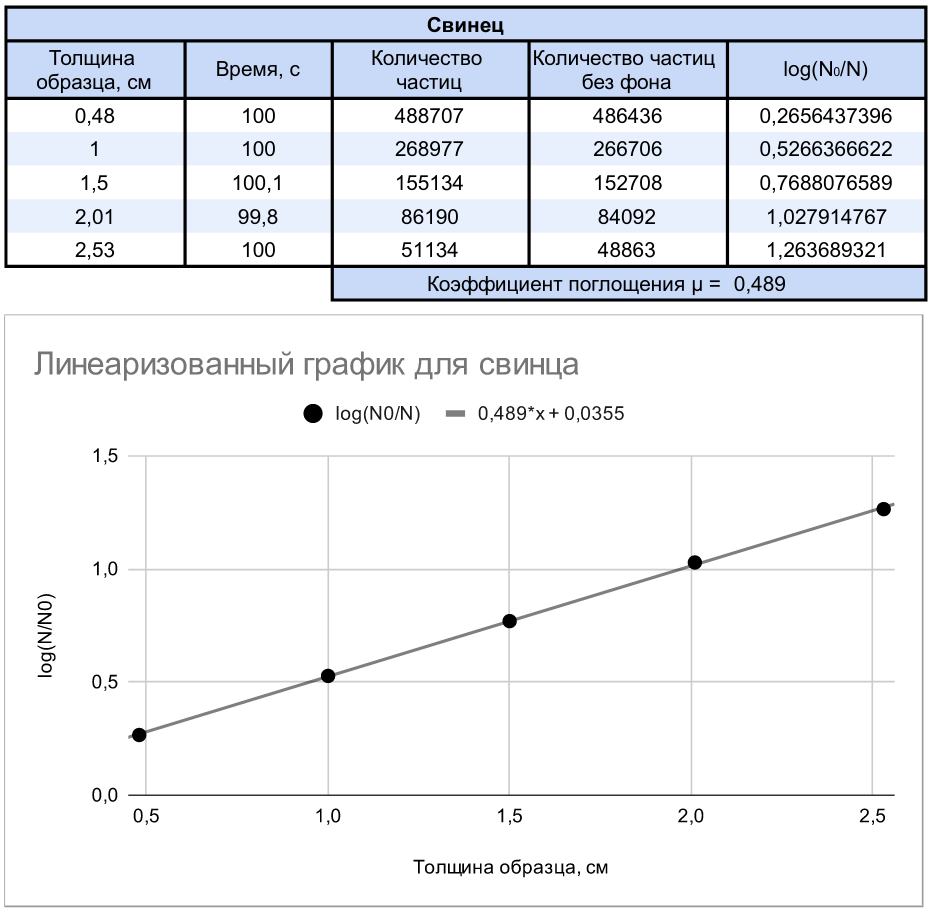
\includegraphics[width = 8.5cm]{pic1.png}}
      Рис 2. График зависимости $log\frac{N_0}{N}$ от толщины образца для
      свинца.
    \end{minipage}
    \hspace{0.5cm}
    \begin{minipage}[h]{0.49\linewidth}
      Табл 2. Количество частиц, прошедших через алюминий за 100 сек.
      \center{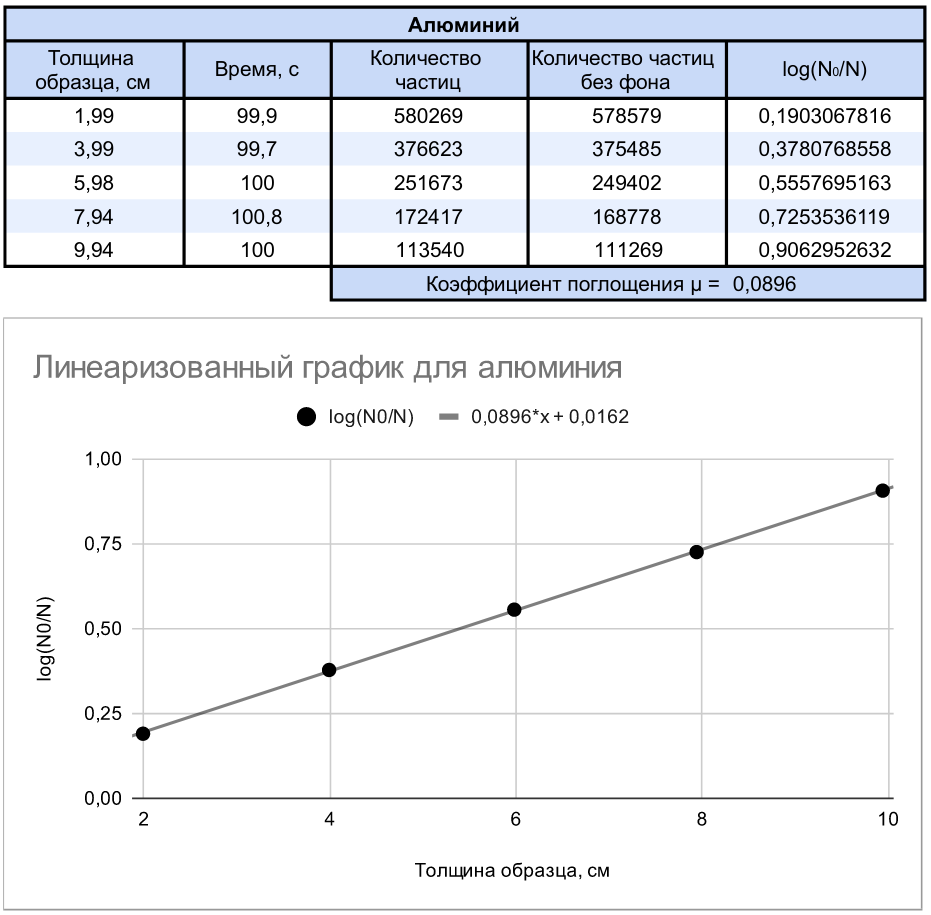
\includegraphics[width = 8.5cm]{pic2.png}}
      Рис 3. График зависимости $log\frac{N_0}{N}$ от толщины образца для
      алюминия.
    \end{minipage}
    \label {fig:plumbum-aluminium}
  \end {figure}

  \begin {figure}[h!]
    \begin{minipage}[h]{0.49\linewidth}
      Табл 3. Количество частиц, прошедших через железо за 100 сек.
      \center{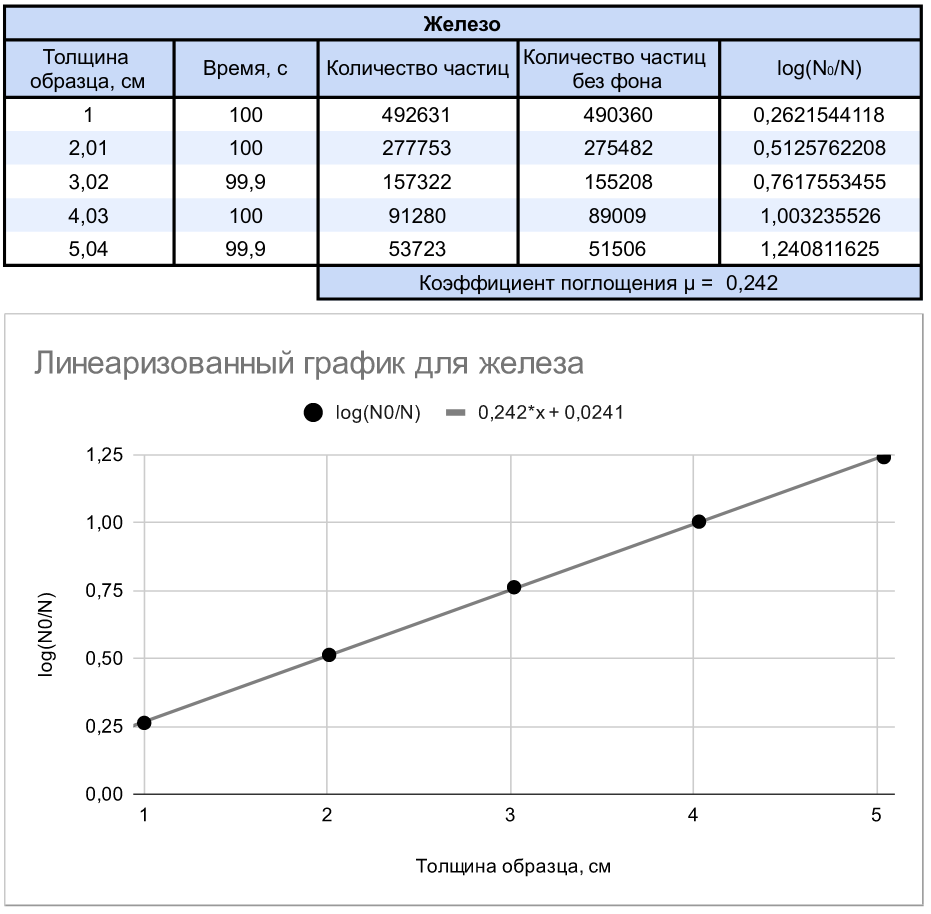
\includegraphics[width = 8.5cm]{pic3.png}}
      Рис 4. График зависимости $log\frac{N_0}{N}$ от толщины образца для
      железа.
    \end{minipage}
    \hspace{0.5cm}
    \begin{minipage}[h]{0.49\linewidth}
      Табл 4. Количество частиц, прошедших через неизвестный за 100 сек.
      \center{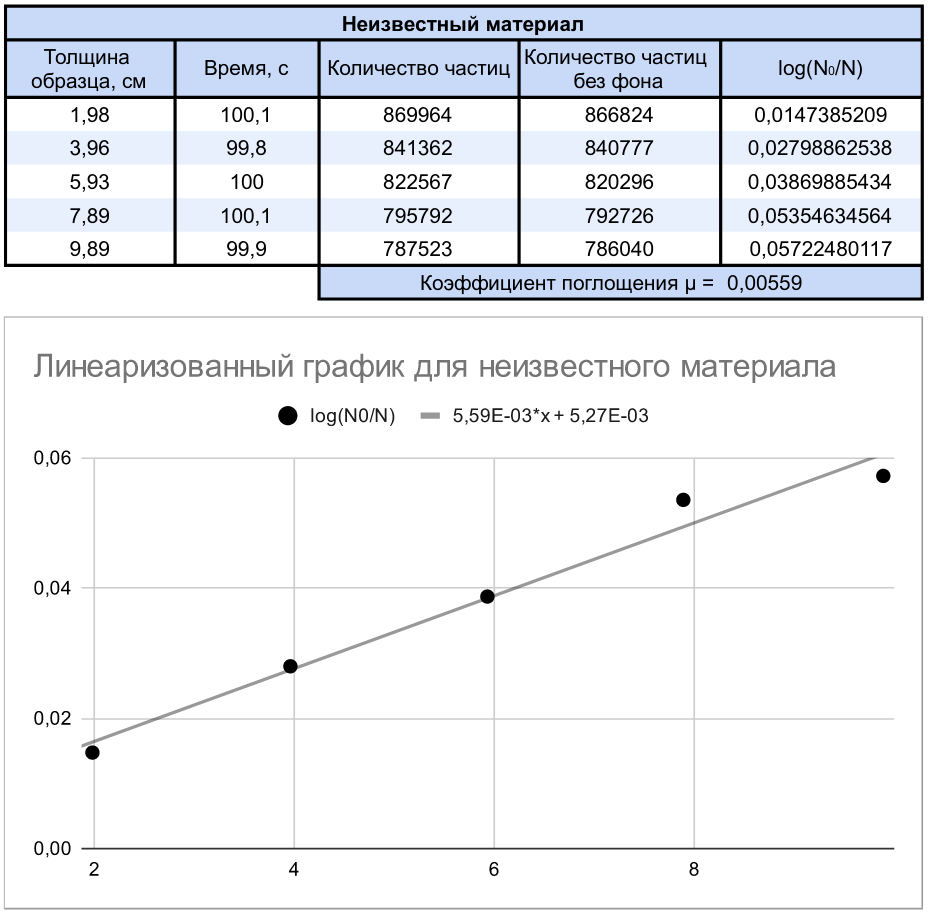
\includegraphics[width = 8.5cm]{pic4.png}}
      Рис 5. График зависимости $log\frac{N_0}{N}$ от толщины образца для
      неизвестного образца.
    \end{minipage}
    \label {fig:ferrum-unknown}
  \end {figure}

  С помощью измеренных значений для $N_0$ и $N$ для каждого образца получили
  зависимости $log\frac{N_0}{N}(l)$, где $l$ - толщина образца.
  Коэффициент наклона прямой будет являться коэффициентом поглощения для
  конкретного образца.

  Таким образом, коэффициенты поглощения будут такими:

  $$
    \mu_{Pb} = 0,489 см^{-1}
  $$
  $$
    \mu_{Al} = 0,0896 см^{-1}
  $$
  $$
    \mu_{Fe} = 0,242 см^{-1}
  $$

  Используя таблицу и график зависимости коэффициента поглощения от энергии
  частиц в пучке выясним, какая энергия была в исследуемом пучке.

  \begin {figure}[h!]
    \begin{minipage}[h]{0.49\linewidth}
      \center{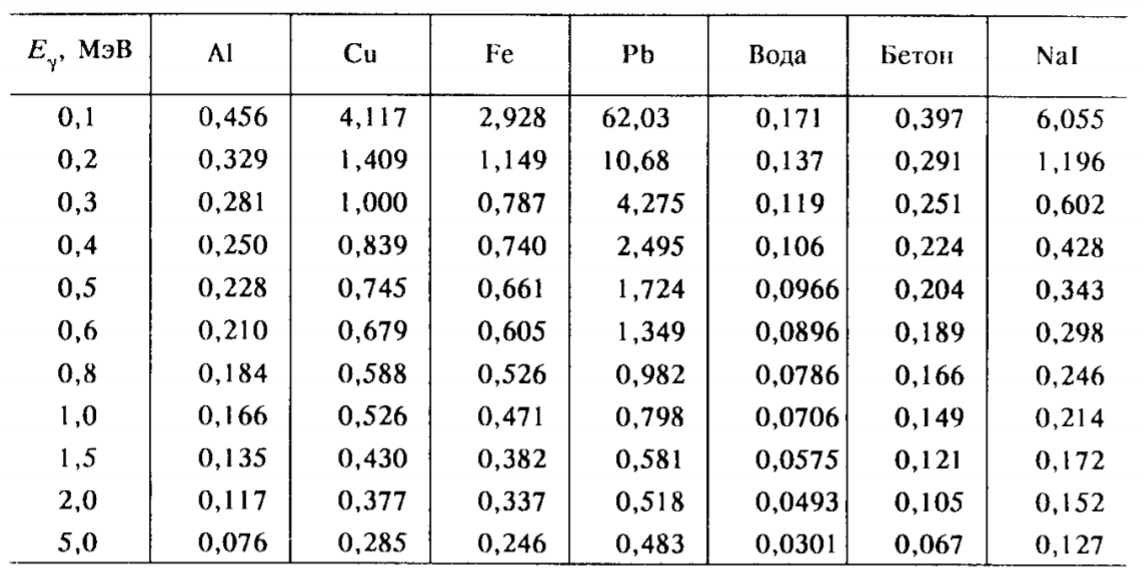
\includegraphics[width = 8.5cm]{pic5.png}}\\
      Рис 6 - Таблица коэффициентов поглощения
    \end{minipage}
    \hspace{0.5cm}
    \begin{minipage}[h]{0.49\linewidth}
      \center{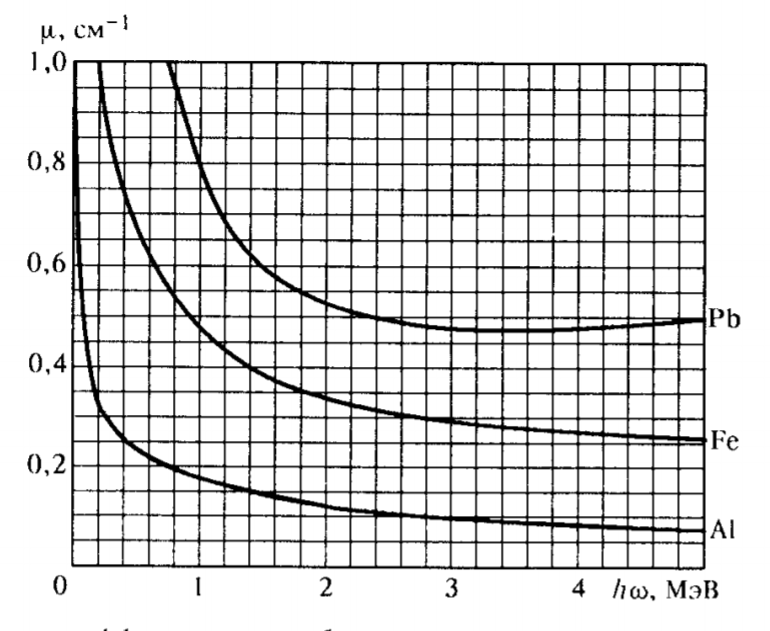
\includegraphics[width = 6.5cm]{pic6.png}}\\
      Рис 7. График зависимости $\mu$ от $h\omega$
    \end{minipage}
    \label {fig:tables}
  \end {figure}

  Согласно таблице легко понять, что энергия пучка находится в пределах от 2
  до 5 МэВ. Для определения более точных значений обратимся к графику.

  Как мы видим, по графику для свинца можно понять, что энергия пучка находится
  в пределах от 2,7 до 4,4 МэВ. Для более точного определения энергии обратимся
  к графику для алюминия. Согласно этому графику энергия пучка равна 3,8 МэВ.
  Однако для железа энергия пучка не совпадает с табличными значениями. Это
  объясняется тем, что в железе зачастую содержаться примеси, которые могут
  влиять на коэффициент поглощения $\gamma$-излучения.

\section{Определение неизвестного материала *}

  Обратимся к рисунку 5 для неизвестного материала. Согласно данным его
  коэффициент поглощения $\mu = 0,00559$, однако идентифицировать материал по
  данному коэффициенту поглощения невозможно. Кроме того из наблюдаемой
  нелинейности на графике можно сделать вывод о неоднородной структуре
  материала. Вероятнее всего этот материал содержит в своей структуре большое
  количество воздуха, который сильно понижает этот коэффициент поглощения.

\section{Вывод}

  Из проведенных измерений можно сделать вывод, что наиболее эффективный
  поглотитель $\gamma$-излучения - это свинец. Однако железо так же показывает
  неплохие характеристики поглощения.



\end{document}
